\documentclass[journal]{new-aiaa}
%\documentclass[conf]{new-aiaa} for conference papers
\usepackage[utf8]{inputenc}

\usepackage{graphicx}
\usepackage{amsmath}
\usepackage{amssymb}
\usepackage{listings}
\usepackage{mathtools}
\usepackage[version=4]{mhchem}
\usepackage[section]{placeins}
\usepackage{siunitx}
\usepackage{longtable,tabularx}
\setlength\LTleft{0pt} 

\title{Convex Programming Approaches to Pinpoint Fuel-Optimal Planetary Landing with Non-Convex Constraints}

\author{Pádraig Lysandrou\footnote{Undergraduate Student, Electrical and Computer Engineering, AIAA Student Member}}
\affil{Cornell University, Ithaca, New York, 14853}

\begin{document}

\maketitle

\begin{singlespace}

\begin{abstract}
In this paper, I present a summary and implementations of work done in convex programming approaches \cite{ploen2007}\cite{enhancements2008}\cite{becet2016}\cite{blackmore2013} to the fuel-optimal powered descent, or "soft-landing", problem. These trajectory optimization problems are nontrivial due to nonconvex control restraints and will be formulated as a finite-dimensional second-order cone program (SOCP). SOCPs are a convex program subclass with efficient solvers that have deterministic convergence properties. I will initially pose and solve a single trajectory optimization program with a time-of-flight search and then explore a successive approach. The successive approach, with nonlinearities, mass-depletion dynamics, and free final time presents a challenge for real-time implementation. To provide a tractable solution we must employ a methods of lossless convexification, linearization, trust regions, and relaxations. Again formulating the problem as an SOCP and initialized with a coarse time-of-flight estimation, it can be solved iteratively, hence successive. These algorithms can be implemented on autonomous real-time systems with powerful modern Interior Point Method (IPM) solvers. This is written as the final project report for Cornell Engineering course ECE5555 Stochastic Systems: Estimation and Control.


\end{abstract}

\section*{Nomenclature}
{\renewcommand\arraystretch{1.0}
\noindent\begin{longtable*}{@{}l @{\quad=\quad} l@{}}
$r$  & position \\
$\textbf{T}$  &Thrust vector (N)\\
$g$   		&Gravity vector of planet $(m/s^2)$ \\
$m(t)$  	&Mass of vehicle\\
$\alpha$ 	&Constant describing mass consumption rate \\
$T_1$   & Lower Thrust Bound\\
$T_2$   & Upper Thrust Bound\\
$\rho_1$   	& Lower Thrust Bound  \\
$\rho_2$	& Upper Thrust Bound\\
$m_{wet}$		& The total mass of the vehicle including propellant\\
$t_f$		& Length of finite time horizon\\
$x$		& Augmented state vector defined as $[r, \dot{r}]^T$\\
$r_z(t)$	& Vertical position \\
$r_x(t)$	& Downrange position \\
$\Theta_{alt}$		& Glideslope constraint \\
$S_j, v_j, a_j$		& Matrices, vectors, and scalars defining convex state constraints\\
$I_{sp}$		& Specific impulse of the rocket engine\\
$u$		& Control acceleration put on by thrusters\\
$\Gamma$		& Slack variable required for convexification \\
$log$		& Natural logarithm\\
$\|x\|$		& Euclidean 2-norm of vector x\\
\end{longtable*}}

\section{Introduction}
In this paper, I present implementations of convex programming algorithms for the powered descent guidance problem. I will focus on these two papers:\cite{ploen2007}\cite{enhancements2008}. Traditional landing algorithms have tolerances of tens of kilometers, where the one presented has tolerances as little as meters. So far, all Mars landings have been for exploration missions with relaxed landing criteria. However, given that landing has gained renewed interest due to privatization and commercialization of space exploration, other techniques are being researched. Having the ability to land near a site of scientific interest, a base, or refueling station is valuable. The convex methods I will present can be used for landing a spacecraft on Mars as well as other planetary bodies like Earth for application in reusable launch vehicles. The ability to soft-land a rocket is fundamentally disruptive to the industry and has already had a huge impact in reducing the cost of getting to space. We have seen companies like SpaceX and Blue Origin make incredible progress with landing reusable vehicles and expect more developments from them in the future.

Every pinpoint landing problem begins with an entry phase where the vehicle descends through an atmosphere to a point where powered descent must begin. Many Mars entry, descent, and landing schemes enter the atmosphere and slow down via parachute. This parachute is then cut away to allow powered descent. With atmospheric qualities being stochastic, the position in which the descent phase must begin is uncertain. Therefore, we would like to look at algorithms which maximize the divert capability of the craft by minimizing the fuel consumption from initial condition to terminal state. We define powered descent guidance as the fuel-optimal trajectory that takes the vehicle at some initial state condition to a prescribed final state in a uniform gravitational field with standard vehicle given thrust magnitude and direction constraints. I will start with the two-dimensional formulation and extend it to three dimensions in my implementation.

The convex optimization framework is exploited because it is conducive of real-time onboard implementation and has guaranteed convergence properties with deterministic criteria. The convex programming algorithm to solve powered descent guidance that I will present has non-convex controls constraints and will be posed as a finite-dimensional SOCP problem. SOCPs have low complexity and can be solved in polynomial time \citep{boyd}. Interior-point numerical methods compute optimal solutions with deterministic stopping criteria and are, again conducive to onboard implementation.  I will summarize the problem given in \citep{ploen2007}, provide a solution, extend it to three dimensions, and then summarize the successive convexification approach found in \citep{becet2016} with my own successive implementation under noise.

\section{The General Problem\citep{ploen2007}}
Given that we will solve our system in two dimensions (x and z), the position and velocity vectors will be of size $\mathbb{R}^2$. We have assumed everything is the the \textit{surface fixed frame.} The translational dynamics of the system are given as
\begin{equation}\label{dynamics1}
\ddot{r}(t)= g + \frac{ T_c (t)}{m(t)}
\end{equation}
\begin{equation}\label{dynamics2}
\dot{m}(t)=-\alpha \lVert T_c (t) \rVert
\end{equation}
Where $\ddot{r}(t)$ $\in$ $\mathbb{R}^2$ is acceleration of the vehicle, $g$ is the gravitational acceleration vector of the planet, $T_c (t)$ is the thrust vector, $m(t)$ is the mass of the vehicle, and $\alpha$ is a positive constant describing the fuel consumption rate. For $n$ identical thrusters each with nominal thrust level $T$ and specific impulse $I_{sp}$ we can denote $\boldsymbol T_c = (nT\cos\phi)\boldsymbol e$ and $\alpha = (I_{sp} g \cos\phi)^{-1}$ as the consumption rate with $\phi$ being the cant angle of each engine. However, moving forward I will assume one engine per spacecraft and, therefore, a cant angle of 0 degrees. 

Engine thrust cannot be continuously throttled down to 0 and therefore has upper and lower bounds 
\begin{equation}
0 < T_1 < T(t) < T_2, \qquad \forall t \in [0,t_f]
\end{equation}
\begin{equation} \label{constraint:1}
\rho_1 \leq \lVert T (t) \rVert \leq \rho_2
\end{equation}
\begin{equation}
\rho_2 > \rho_1 > 0
\end{equation}
Where $\rho_1$ is the deepest throttle and $\rho_2$ is the nominal largest thrust value. The final time is denoted by $t_f$. Note that eqn.\ref{constraint:1} defines a nonconvex region in the control space. We must also provide the initial conditions: $m(0) = m_{wet}$, $x(0) = x_0$, $x(tf) = 0$, where $x$ denotes the state. The value $m_{wet}$ is the wet mass of the rocket. This means the mass of the structure, avionics, and other non-consumables plus the mass of the fuel in the tanks.  The state is constructed as such: $x = [r \quad \dot{r}]^T$. We also assume that $r_z (t) > 0, \quad \forall t \in [0,t_f)$ which is to say that the vehicle cannot travel through the ground.

Another set of constraints that we must consider are those imposed upon the system by instruments and sensors. For example, when landing on a planetary body without global positioning, terrain relative navigation might be used and restrict the attitude of the vehicle. For this we implement what is called the glideslope constraint.
\begin{equation}
\Theta_{alt} = \arctan{\frac{r_z(t)}{r_x(t)}}
\end{equation}

Additionally, it is assumed that constraints take the following affine form:
\begin{equation}
\|S_jx(t)-v_j\| + c_j^Tx(t)+a_j\leq 0
\end{equation}
where $S_j \in \mathbb{R}^{n_j*4} $, $c_j \in \mathbb{R}^4$, $n_j\leq 4$, $v_j \in \mathbb{R}^n_j$, and $a_j \in \mathbb{R}$. Similarly we can express the glideslope constraint like
\begin{equation}
\|Sx\| + c_j^Tx\leq 0
\end{equation}
where

\[
S = 
\begin{bmatrix}
1 &0 &0 &0 \\
0 &1 &0 &0
\end{bmatrix}, \qquad
c = 
\begin{bmatrix}
-\tan{\Theta_{alt}} &0 &0 &0 \\
\end{bmatrix}^T
\]

So we can now pose
\begin{align*}
 \textbf{Problem 1:} \\
 \quad \max_{t_f, T} m(t_f) = \min_{t_f, T}\int^{t_f}_0 \|T(t)\| dt \\
 \textbf{Subject to:} \\
 \quad \ddot{r}(t)= g + \frac{\boldsymbol T_c (t)}{m(t)}, \quad \dot{m}(t)=-\alpha \|T_c (t)\| \\
 \rho_1 \leq \lVert T (t) \rVert \leq \rho_2, \quad  r_z(t) \leq 0 \\
 \|S_jx(t)-v_j\| + c_j^Tx(t)+a_j\leq 0, \quad j = 1,...,n_s \\
 m(0) = m_{wet}, r(0) = r_0, \dot{r}(0) = \dot{r_0}, r(t_f) =\dot{r}(t_f) = 0
\end{align*}


\section{Convexification of the Control Magnitude Constraint}
I will now introduce a modified version of Problem 1:
\begin{align*}
 \textbf{Problem 2:} \\
 \min_{t_f, T, \Gamma}\int^{t_f}_0 \|\Gamma(t)\| dt \\
 \textbf{Subject to:} \\
 \ddot{r}(t)= g + \frac{\boldsymbol T_c (t)}{m(t)}, \quad \dot{m}(t)=-\alpha \|\Gamma (t)\| \\
 \|T(t)\| \leq \Gamma(t) \\ 
 \rho_1 \leq \Gamma(t) \leq \rho_2, \quad  r_z(t) \leq 0 \\
 \|S_jx(t)-v_j\| + c_j^Tx(t)+a_j\leq 0, \quad j = 1,...,n_s \\
 m(0) = m_{wet}, r(0) = r_0, \dot{r}(0) = \dot{r_0}, r(t_f) =\dot{r}(t_f) = 0
\end{align*}
This is derived by introducing $\Gamma$ as a slack variable to the initial problem. $\Gamma$ replaces $\|T\|$ with an additional constraint $\|T(t)\| \leq \Gamma(t)$. Because this problem is a relaxation of the initial problem, Problem 1 defines a feasible solution of Problem 2. However, a feasible solution for problem 2 does not necessarily define one for Problem 1. Lemma 1 of \citep{ploen2007} shows that the optimal solution to Problem 2 also is a feasible solution of Problem 1. This is done by using the Hamiltonian of Problem 2 and using the necessary conditions for optimality, pointwise maximum principle, and the transversality condition. This paper shows, with lemma 1, that modified constraints of Problem 2, namely the scalar slack variable $\Gamma$ convexifies Problem 1. The lemma states that if there is an optimal solution to Problem 2, then there also exists one for Problem 1, and it can be found from the optimal solution of Problem 2. We also see that that the admissible set of controls for the second problem are within the set of admissible controls for the first. Together this means that Problem 2 can be solved with convex control constraints in order to find a solution to the nonconvex Problem 1. 

\begin{figure}[hbt!] 
\centering
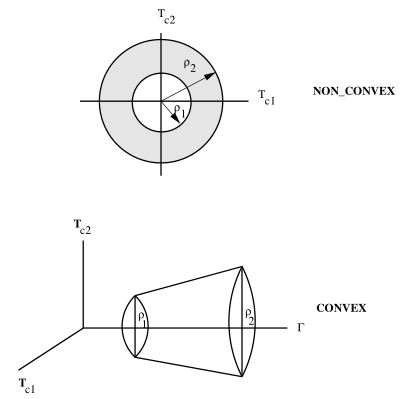
\includegraphics[scale=0.25, width=.5\textwidth]{convexification.PNG}
\caption{Problem 1 to Problem 2 convexification of the thrust constraint. From \citep{ploen2007}}
\label{fig:convexif}
\end{figure}

See Fig. \ref{fig:convexif} to see how the original nonconvex annulus turns into a three-dimensional convex cone. The \citep{ploen2007} paper gives a optimal solution existence proof and continues onto a change of variables step which will make construction of the algorithm much simpler.

\subsection{Change of Variables}
A change of variables will allow for a much cleaner numerical algorithm for expanding Problem 2 into the third form which will be a continuous time SOCP. Let us perform
\begin{align}
\sigma = \frac{\Gamma}{m} \\
u = \frac{T}{m}
\end{align}
and consequently the dynamics change
\begin{align}
\ddot{r}(t) = u(t) + g \\
\frac{\dot{m}(t)}{m(t)} = -\alpha\sigma(t) \\
\text{and clearly } m(t)= m_0\exp\big[-\alpha \int^{t_f}_0 \sigma(t)d\tau \big]
\end{align}

Therefore we must minimize the integral term in the last mass dynamical equations. The original constraints the follow that
\begin{align}
\|u(t)\| \leq \sigma(t), \quad \forall t \in [0,t_f] \\
\frac{\rho_1}{m(t)} \leq \sigma(t) \leq \frac{\rho_2}{m(t)}, \quad \forall t \in [0,t_f] 
\end{align}

This inequality now describes a convex set. However, when we consider $m$ by itself to be variable of the problem, these inequalities become bilinear and do not define a convex region. We will now introduce $z$ to resolve this issue and convexify these inequalities. Lets define $z = \log{m}$. And then the mass depletion rate now becomes $\dot{z}(t) = -\alpha\sigma(t)$.
The inequalities now become
\begin{equation} \label{convinq}
\rho_1\exp{(-z(t))} \leq \sigma(t) \leq \rho_2\exp{(-z(t))}. \quad \forall t \in [0, t_f]
\end{equation}

The left side of the inequality in eqn. \ref{convinq} defines a convex feasible region, but the right part does not. We will now use a Taylor expansion of the exponential to achieve second-order cone and linear approximations to be used in our problem. The first part of this eqn. \ref{convinq} can be approximate by the first three terms of the series, or second-order cone:
\begin{equation}
\rho_1 \exp(-z_0) \Big[ 1-(z-z_0)+\frac{(z-z_0)^2}{2} \Big] \leq \sigma
\end{equation}
Where $z_0$ is a given constant. The right side of the inequality can be linear, or the first two terms of the Taylor expansion. Therefore
\begin{align}
\sigma \leq \rho_2 \exp(-z_0) \big[ 1-(z-z_0)\big] \\
\text{with } \mu_1 = \rho_1 \exp(-z_0), \text{and } \mu_2 = \rho_2 \exp(-z_0)
\end{align}
We now have a second order cone formulation where $z_0(t) = \log(m_{wet}-\alpha\rho_2t)$ where $z_0(t)$ serves as a lower bound on $z(t)$ at each time. We must now ensure that $z(t)$ is constrained properly with
\begin{equation}
\log(m_{wet}-\alpha\rho_2t) \leq z(t) \leq \log(m_{wet}-\alpha\rho_1t) 
\end{equation}

Let us know pose the third problem, substituting in these simplifications, which remains continuous:
\begin{align*}
 \textbf{Problem 3:} \\
 \min_{t_f, u,\sigma}\int^{t_f}_0 \sigma(t) dt \\
 \textbf{Subject to:} \\
 \ddot{r}(t)= u(t) +g, \quad \dot{z}(t)=-\alpha \sigma(t) \\
 \|u(t)\| \leq \sigma(t) \\ 
 \mu_1(t)\Big[ 1-(z-z_0)+\frac{(z-z_0)^2}{2} \Big] \leq \sigma \leq \mu_2(t)\big[ 1-(z-z_0)\big] \\
 \log(m_{wet}-\alpha\rho_2t) \leq z(t) \leq \log(m_{wet}-\alpha\rho_1t) \\
 \|r_x(t)\| \leq \beta r_z(t) \\
 m(0) = m_{wet}, r(0) = r_0, \dot{r}(0) = \dot{r_0}, r(t_f) =\dot{r}(t_f) = 0
\end{align*}

Note that we have replaced the general affine constraint form with the glideslope constraint, where $\beta$ is the defined slope.
\clearpage

\section{Discretization}
Discretization must occur for implementation in computer program. We base this on a piecewise linear control input for different time intervals. This means that for $\Delta t > 0$, and for each instance $t_k = k\Delta t, \forall k = 0,...,N$. Therefore we replace the continuous time with

\begin{align}
u(t) = u_k + (u_{k+1} - u_k)\tau \\
\sigma(t) = \sigma_k + (\sigma_{k+1} - \sigma_k)\tau \\
\text{where } \tau = \frac{t - t_k}{ \Delta t}, \quad \forall t \in [t_k,t_{k+1}), \quad k = 0,...,N-1
\end{align}

Using this discretization, we present Problem 4:

\begin{align*}
 \textbf{Problem 4:} \\
 \min_{u_0 ... u_N, \sigma_0 ... \sigma_N} -z_N \\
 \textbf{Subject to: for } k = 0,...,N,\\
r_{k+1} = r_k + \frac{\Delta t}{2}(\dot{r_k} + \dot{r}_{k+1}) + \frac{\Delta t^2}{12}(u_{k+1}-u_k) \\
\dot{r}_{k+1} = \dot{r}_k + \frac{\Delta t}{2}(u_k + u_{k+1}) - g\Delta t \\
z_{k+1} = z_k - \frac{\alpha \Delta t}{2}(\sigma_k + \sigma_{k+1}) \\
\|u_k\| \leq \sigma_k \\ 
 \mu_{1,k}(t)\Big[ 1-(z_k-z_{0,k})+\frac{(z_k-z_{0,k})^2}{2} \Big] \leq \sigma \leq \mu_{2,k}(t)\big[ 1-(z_k-z_{0,k})\big] \\
 \log(m_{wet}-\alpha\rho_2k\Delta t) \leq z_k \leq \log(m_{wet}-\alpha\rho_1k\Delta t) \\
 \|r_x(t)\| \leq \beta r_z(t) \\
 m(0) = m_{wet}, r(0) = r_0, \dot{r}(0) = \dot{r_0}, r(t_f) =\dot{r}(t_f) = 0, z_0 = log(m_{wet}), N\Delta t = t_f
\end{align*}

We now have the general lossless-convexified algorithm and can use vehicle parameters to generate trajectories.

\section{2D Mars Landing Divert for Small Single-Engined Vehicle}
I have now implemented this algorithm in MATLAB using the CVX package to define the convex problem. I use the SEDUMI solver. In Fig.\ref{fig:param} we see the parameters that I have given the vehicle. I have modeled these off of parameters similar to Masten Space System's vertical takeoff and vertical landing class of vehicles. The specific impulse reflects that of an ethanol liquid oxygen rocket engine, as well as the throttleability of their engine. Notice that the gravity vector reflects that of Mars. I have also limited the maximum thrust vector control angle to 25 degrees as a constraint on the thrust vector. This is a feasible upper limit for agile landing thrust vector control systems. Notice the initial conditions placed on the position and velocity. These values are consistent with those  of Mars entry after the drag/parachute phase. The trajectory in Fig.\ref{fig:traj} shows how the vehicle overshot the target during the entry phase and how it works its way back towards the landing site. Keep in mind that the $t_f$ in this situation is static at 100 seconds and is not necessarily globally optimal because we have yet to implement the time-of-flight search. Fig. \ref{fig:posvel} shows the position and velocity of the vehicle along the path. Additionally, I have rewritten the vehicle parameters, environmental parameters, and initial conditions to simulate the re-entry of SpaceX's Falcon 9 vehicle as it approaches the landing barge. Note that this was done as a demonstration and does not accurately represent their implementation as it does not include aerodynamic control surfaces or disturbances.


\section{3D Implementation of the Landing Algorithm}
Now that I have shown the mathematical derivation for the two dimensional case, I will extend it to three dimensions in the MATLAB simulation. This was very simple as I augmented the dynamics, gravity, and input vectors. The thruster now has two rotational degrees of freedom. I also re-derived the glideslope constraint and thrust vector control constraints for the new degree of freedom. I will include plots of trajectories using both the 3D algorithm and the time-of-flight search algorithm in the appendix for brevity. I will reference them in the following section.


\section{Time-of-Flight (TOF) Search}
Now that we can solve the landing problem with static final time, we must perform this SOCP multiple times, performing a linear search, with multiple times in mind to find the global minimum fuel consumption. For example, even though a feasible solution to the convex problem exists with a final time of 150 seconds, it might be suboptimal to the SOCP solution generated with a 148 second time-of-flight. Therefore we must perform an outer iteration of the time horizon to find the globally optimal value corresponding to total minimum fuel consumption.

We will use the Golden search algorithm, a nonlinear program, to determine this optimal time-of-flight value $t_f^\star$. The minimum fuel is a unimodal function of time and has a global minimum and we can perform another optimization to find the optimal value. Therefore, it can be said that we are performing an outer search, where each value of the search is calculated by a convex optimization problem. This is the most time intense portion of this approach and is the least conducive towards onboard implementation. Additionally, it should be noted that finding the proper upper and lower bounds for $t_f$ is nontrivial and a problem on its own.

For the sake of complexity abstraction, I have decided to use MATLAB's $fminbnd$ function to perform this search for me. This function performs:

\begin{equation}
\min_{t_f} lander(t_f, r_0, v_0, r_N, v_N, params, N), \quad \forall t_{min} \leq t_f \leq t_{max}
\end{equation}

\begin{figure}[!htb] 
  \centering
  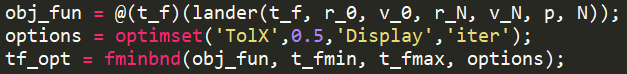
\includegraphics[width=.65\textwidth]{fminbnd.PNG}
  \caption{Implemented in MATLAB}
  \label{fig:fmin}
 \end{figure}
 
 Fig. \ref{fig:fmin} shows the MATLAB implementation referencing the 3D landing algorithm function \texttt{lander.m}. The inputs to the function are the terminal time value, the initial state conditions, terminal state conditions, the vehicle parameters stored in struct \texttt{p}, and the granularity of the trajectory generation $N$. The lander function outputs the mass used, state information, as well as control effort vector $u$. The \texttt{fminbnd} function finds the minimum output of the function for varying the terminal time input value. This means that it takes the Euclidean norm of \texttt{lander}'s output vectors and then compares them along its search to find the global minimum. For my experimentation, I have not attempted to derive proper minimum or maximum values for this iteration. Instead, if the individual optimization is infeasible, I set the output consumption value to an arbitrarily large value. This allows me to set the minimum time to zero and the maximum time to an arbitrary value that I know is too large through experimentation.

An output of this search algorithm can be seen in Fig. \ref{fig:optimn}. The $x$ column indicates the terminal time values that have been tested while the $f(x)$ column indicates the total mass consumed in that iteration. Notice that for the infeasible problems, the mass is 2000 which is the arbitrarily large value I have given it. It is the sum of the initial dry and fuel masses. Notice that the search algorithm starts using the golden search method in the initial iterations and then uses a parabolic algorithm to reach the tolerance setting.

This TOF search took 177.585254 seconds to perform. This can drastically be decreased by minimizing the granularity of the calculation and decreasing the minimum and maximum terminal time boundaries.

\section{The Successive Convexification Approach}
I will now show my efforts in creating a successive algorithm that successively solves the convex problem at each time step under estimation noise. This effectively makes the system closed-loop as it recalculates the trajectory after each input and estimation value. This is, again, another part that is very hard to implement online but can be done with proper computing power.

\begin{figure}[!htbp] 
  \centering
  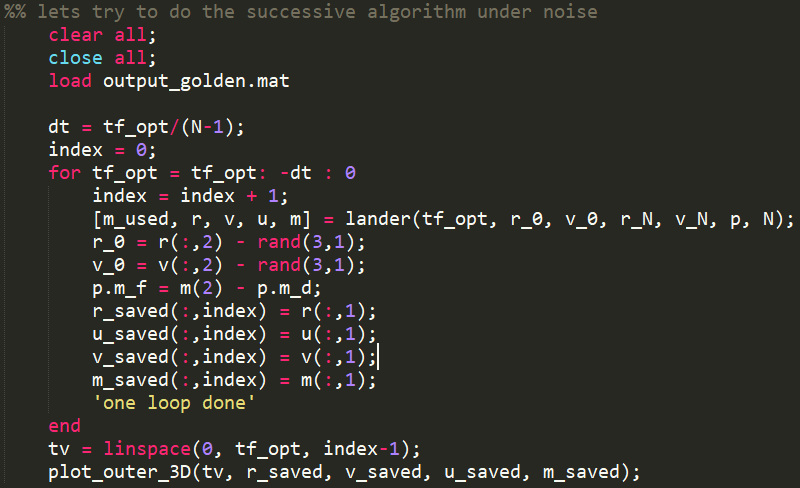
\includegraphics[width=.75\textwidth]{succme.PNG}
  \caption{Successive Algorithm}
  \label{fig:succ}
\end{figure}

In Fig. \ref{fig:succ} we see the general layout of the successive algorithm. First we clear all of the available information and load the output from the TOF search algorithm. The only data we really use are the vehicle parameters, optimal terminal time value, and other constants. We define the time step by the optimal terminal time divided by the total granularity. We then iteratively solve the \texttt{lander.m} algorithm with mass depletion dynamics additive noise to the state vectors. The \texttt{randn} function in MATLAB returns a random scalar drawn from the standard normal distribution. This is not how aerodynamic uncertainty works, but I am doing this for simplicity and can make it more complicated later. Note that the struct value of fuel mass consistently changes with the known consumption from the last iteration. I then save the values for display later.

Please see Fig. \ref{fig:unfin} and Fig. \ref{fig:unfin2} for the outputs of the 3D successive algorithm for the originally posed Mars Landing problem. You will see that the trajectory generation is unfinished. This is unfortunately because of my own time constraints and a small glitch. From the data shown, the simulation runs very well and stays within all given constraints. At the last time point shown, the vehicle had only consumed about 150kg of propellant with an additional 350 to its disposal. In optimal conditions it should only consume 315 kg given by Fig. \ref{fig:optimn}. Therefore, the unfinished trajectory and data look very correct and follow the optimal path. Therefore it looks promising and robust under noise. I will continue to work on this solution after the end of the course. 


\section{Future Work and Implementation of Successive Algorithm}
After the completion of ECE5555, I plan on completing and polishing up my successive solution. I also plan on autocoding my algorithm in C/C++ using the CVXgen tool. I will run it on a small embedded Linux platform and see what kind of cycle times I can get as it converges to an optimal trajectory. Additionally, I plan on implementing an offline version of the algorithm on a small electric-ducted-fan vehicle that will simulate the inertial properties of a rocket body. I will attempt to land this vehicle with some initial conditions.



\section{Conclusion}
I have presented an algorithm that can generate trajectory and control inputs for fuel-optimal landings. This can be used as an offline optimizer or used online in a successive fashion where the optimal time-of-flight is converged upon. This algorithm has many uses and is useful in the landing of reusable launch vehicles back to Earth and research vehicles on other planets. Implementation of algorithms like this have already had a profound impact on the aerospace industry and are the key to reducing cost to space access. I have shown that a successive approach, effectively closed loop, is robust under noise. Overall, I have learned an incredible amount working on this project in my own time and will continue working on it going forward. I would like to thank Prof. Eilyan Bitar for his help and guidance during this project.

\appendix
\section{APPENDIX}
\subsection{Problem 4 CVX Program}
\scriptsize
\begin{lstlisting}[language=MATLAB]
cvx_begin
	variables u(2,N) z(1,N) s(1,N) r(2,N) v(2,N)
	minimize(-z(N))			% objective function
	subject to 				% constraints and dynamics
		r(:,1) == r_0;		% position IC
		v(:,1) == v_0;		% velocity IC
		r(:,N) == r_N; 		% position TC
		v(:,N) == v_N;		% velocity TC
		z(1) == log(m_t);	% mass IC
		r(2,:) >= 0;		% ground clearance
		u(2,:) >= s.*cos(degtorad(tv_max));	% thrust vector control constraint
		r(1,:) <= r(2,:)/tan(degtorad(gs));	% glide slope
        z(:) >= 0;
		for  k = 1:N-1
			r(:,k+1) == r(:,k) + ((dt/2)*(v(:,k) + v(:,k+1))) +(((dt^2)/12)*(u(:,k+1) - u(:,k)));
			v(:,k+1) == v(:,k) + ((dt/2)*(u(:,k) + u(:,k+1))) +(g_plan*dt);
			z(1,k+1) == z(1,k) - (((a*dt)/2)*(s(1,k) + s(1,k+1)));
        end
		for k=1:N
			norm(u(:,k)) <= s(1,k);
			z_0 = m_t - (a*rho2*dt*(k-1));
			m_1 = rho1/z_0;
			m_2 = rho2/z_0;
			z1 = log(m_t-(a*rho1*dt*(k-1)));	
			z0 = log(z_0);
			z(1,k) >= z0;
			z(1,k) <= z1;
			s(1,k) <= m_2*(1 - (z(1,k) - z0));
			s(1,k) >= m_1*(1 - (z(1,k) - z0) + (((z(1,k) - z0)^2)/2));
        end
cvx_end
\end{lstlisting}
\normalsize

\subsection{2D Figures for Mars Landing With Glideslope Constraint}
  \begin{figure}[!htb] 
  \centering
  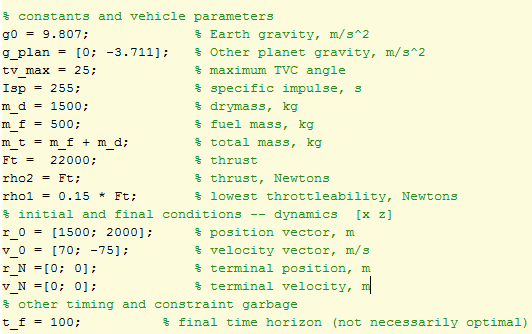
\includegraphics[width=.6\textwidth]{marsparam.PNG}
  \caption{Single engined small Mars vehicle parameters.}
  \label{fig:param}
  \end{figure}
  \begin{figure}[!htb] 
  \centering
  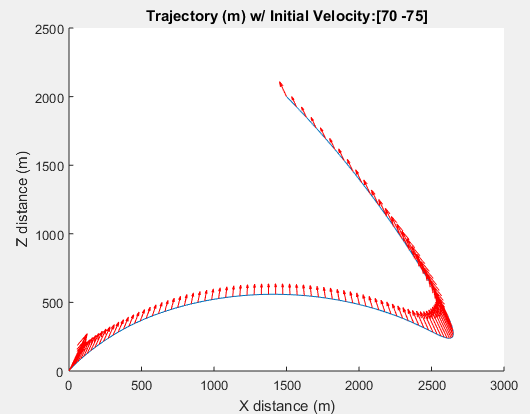
\includegraphics[width=.6\textwidth]{marstraj.PNG}
  \caption{Single engined small Mars vehicle trajectory generated with static finite time. This shows the magnitude and direction of the thrust as well as outlines the path of movement.}
  \label{fig:traj}
  \end{figure}
  \begin{figure}[!htb] 
  \centering
  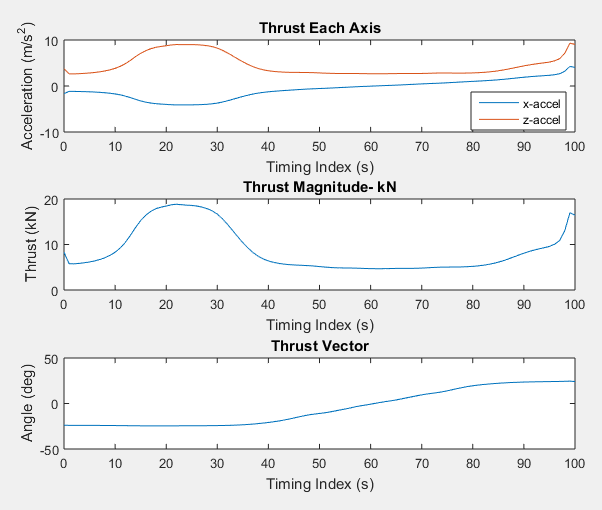
\includegraphics[width=.6\textwidth]{marsposvel.PNG}
  \caption{Single engined small Mars vehicle subplot array shows the position and velocity of the lander along the trajectory.}
  \label{fig:posvel}
  \end{figure}

\subsection{2D Earth Landing of Falcon 9 Without Glideslope Constraint}
\begin{figure}[!htb] 
\centering
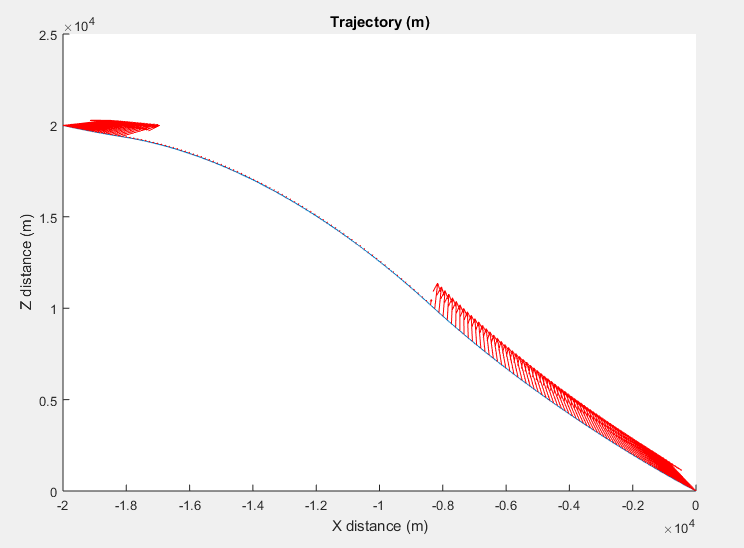
\includegraphics[width=.6\textwidth]{falcon.PNG}
\caption{Earth Landing Trajectory of SpaceX's Falcon 9 first stage rocket as it approaches the barge for landing.}
\label{fig:falcon}
\end{figure}

\subsection{3D Mars Landing with Glideslope Constraint, Same Vehicle Parameters as \ref{fig:param}, and TOF search}
\begin{figure}[!htb] 
\centering
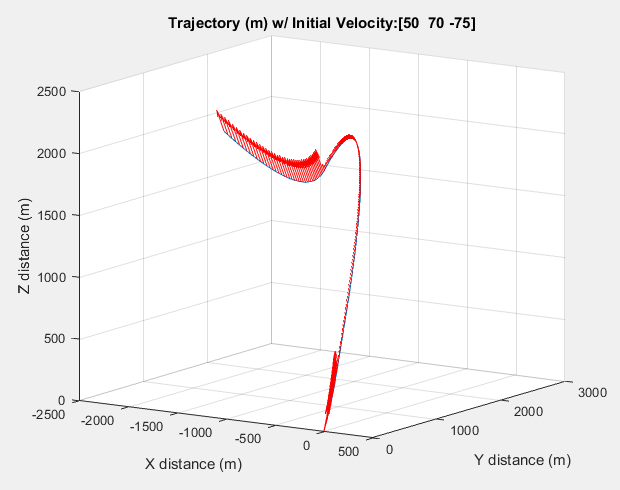
\includegraphics[width=.8\textwidth]{3Dtraj.PNG}
\caption{3D Mars landing trajectory with glideslope constraints and optimal terminal time given from TOF search.}
\label{fig:optimn}
\end{figure}
\begin{figure}[!htb] 
\centering
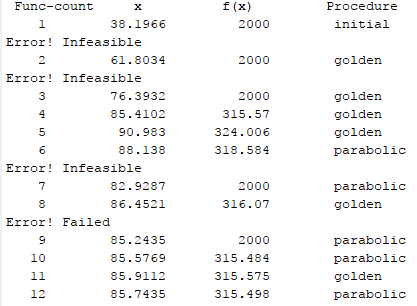
\includegraphics[width=.6\textwidth]{optimn.PNG}
\caption{Output from the fminbnd linear search. Notice that it starts using the golden search algorithm in the initial iterations and then uses a parabolic algorithm to reach the tolerance setting.}
\label{fig:optimn}
\end{figure}

\subsection{Successive Algorithm Figures}

\begin{figure}[!htb] 
\centering
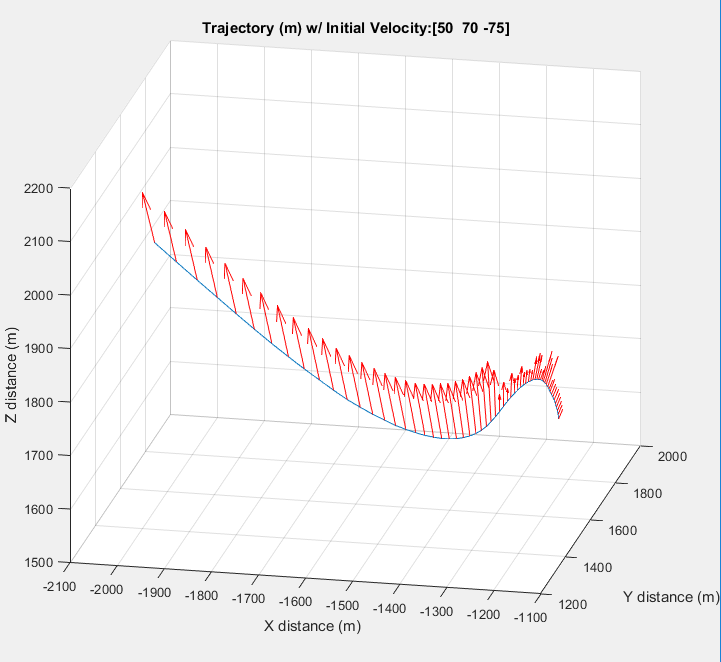
\includegraphics[width=.75\textwidth]{unfin.PNG}
\caption{This is the unfinished 3D trajectory generated by the successive algorithm and noise initial conitions.}
\label{fig:unfin}
\end{figure}

\begin{figure}[!htb] 
\centering
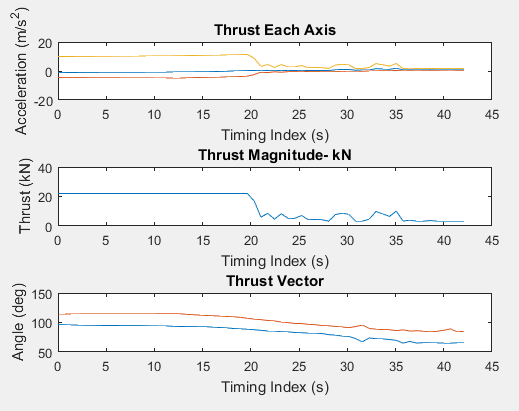
\includegraphics[width=.75\textwidth]{unfin2.PNG}
\caption{These are the control inputs from the unfinished 3D trajectory generated by the successive algorithm}
\label{fig:unfin2}
\end{figure}



\clearpage
\bibliography{sample}

\end{singlespace}
\end{document}
